\chapter{Generator parameters and architecture}

In logic it is common to characterize element by its name and arity (if applicable), but in implementation name of element can be filled any time and besides arity, often argument type is also important. 

% \begin{itemize}
  % \item element name is not important
  % \item types of child elements is important
% \end{itemize}

% See table \ref{tab:signatureComparison} for more details.
%
% \begin{table}
  % \centering
  % \footnotesize
  % \begin{tabularx}{\textwidth}{|c|X|X|}
    % \hline
    % FOL element & Unique element in mathematical sense & Unique element as signature \\
    % \hline
    % Variable & by name and scope $V1$, $V2, \dots$ & there is only one signature for variable \\
    % \hline
    % Functor & by name and arity $f/0$, $f/1, \dots$ & by types of arguments $f(Variable)$, $f(functor), \dots$ \\
    % \hline
    % Predicate & by name and arity $p/0$, $p/1$, \dots & by types of arguments $p(Variable)$, $p(functor), \dots$ \\
    % \hline
    % Atom & by connective and operands $p/0$, $f/1 = V, \dots$ & by connective and operands signatures $p(Variable)$, $f(Variable) = f(Functor), \dots$ \\
    % \hline
  % \end{tabularx}
  % \caption{Comparison of how elements of FOL in sense of math and signature. Elements not included here simply does not make sense to have signature}
  % \label{tab:signatureComparison}
% \end{table}

Abstract syntax tree of \gls{FOL} is implemented in the same way as mathematical definition, see picture \ref{pic:fol_elements_class_diagram}.

\begin{figure}[h]
\begin{centering}
  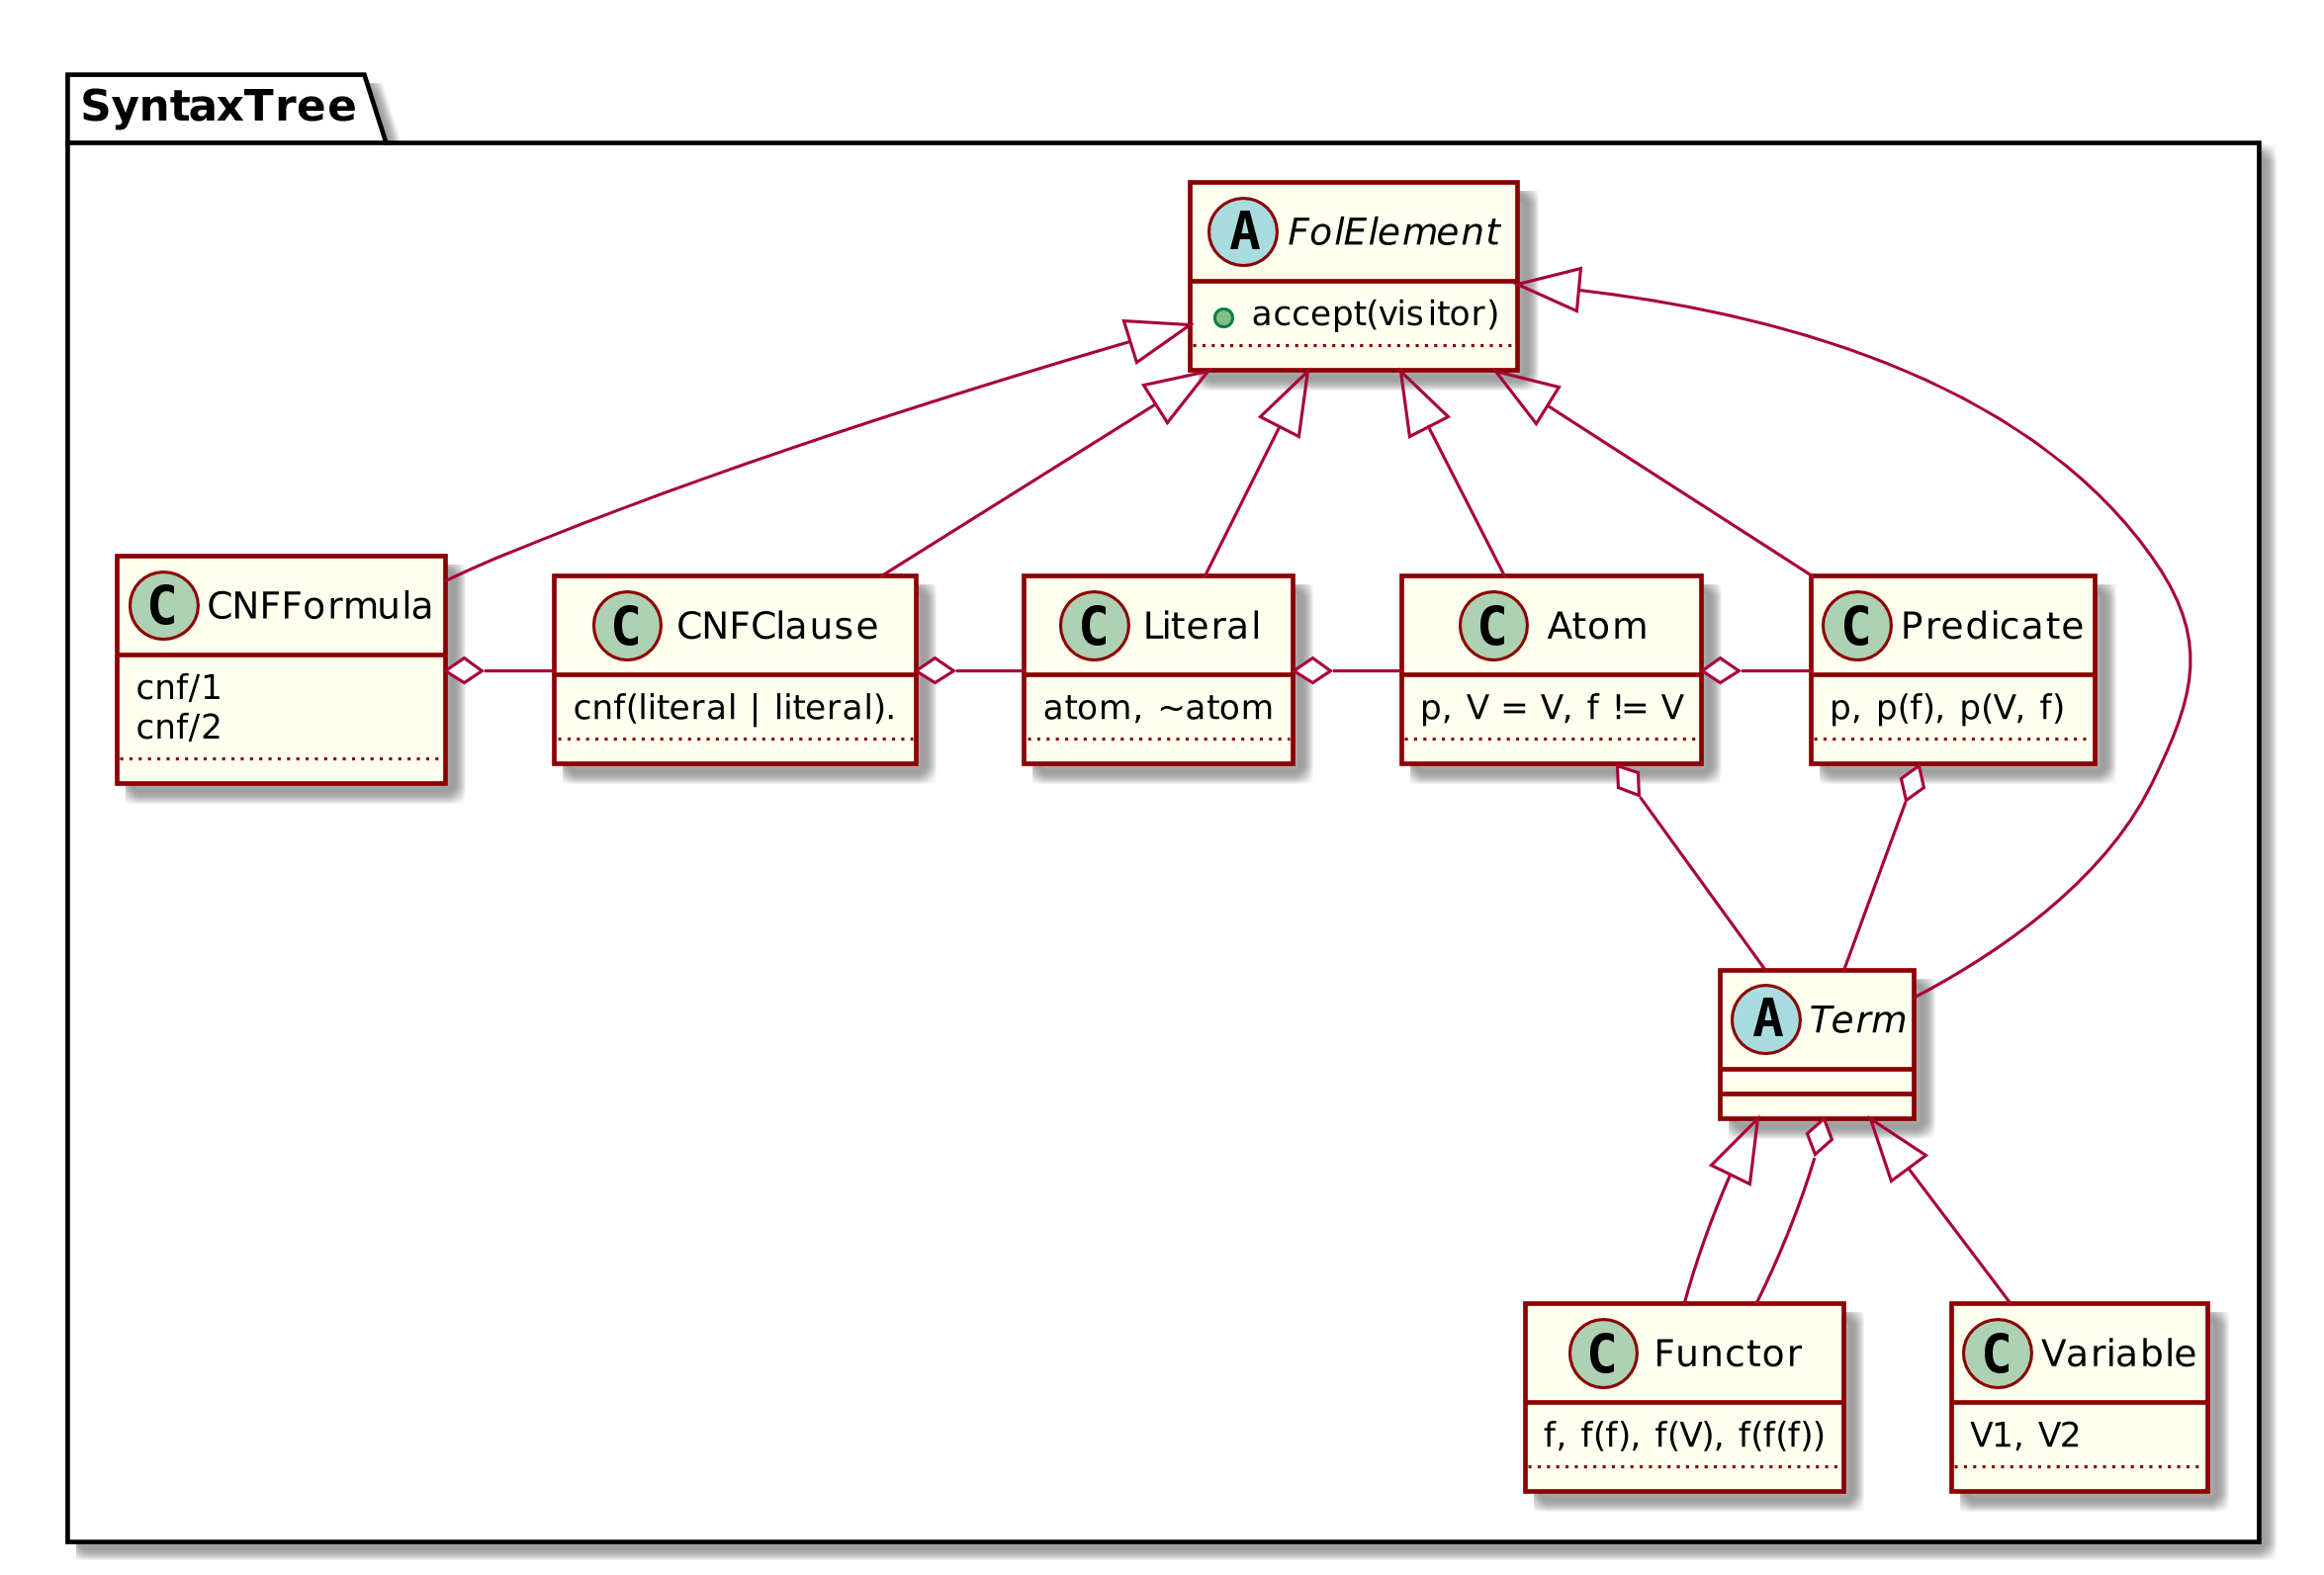
\includegraphics[width=\textwidth]{logic-formula-generator/fol/cnf_fol_elements.png}
  \caption{Class diagram for internal representation of first order logic elements}
  \label{pic:fol_elements_class_diagram}
\end{centering}
\end{figure}

\section{CNF Generator parameters}

User defines generator in 2 steps.
\begin{enumerate}
  \item \textbf{General setting for generated formula}

    In this step user defines set of allowed \gls{FOL} elements:
    \begin{itemize}
      \item set of variable names $\{'v1','v2',\dots\}$
      \item set of functor names $\{'f1','f2',\dots\}$
      \item set of predicate names $\{'p1','p2',\dots\}$
      \item set of allowed functor arities $a_f = \{0, 1, 2,\dots\}$
      \item maximum recursion depth $n$ for functors
      \item set of allowed predicate arities $a_p = \{0, 1, 2,\dots\}$
      \item set of atom allowed connectives, that is no connective or/and any subset of $AllowedConnectives = \{=, !=, \emptyset\}$
      \item set of allowed clause lengths $AllowedClausesLengths = \{1,2,\dots\}$
      \item amount of literals to be negated
    \end{itemize}

  \item \textbf{How many instances of elements are allowed}

    In this step user defines what properties formula should have:
    \begin{itemize}
      \item formula contains from $c_{min}$ to $c_{max}$ clauses
      \item formula contains from $l_{min}$ to $l_{max}$ literals
    \end{itemize}

\end{enumerate}

\section{Basic algorithm}

\begin{enumerate}
  \item Resolve user constraints \ref{sec:ResolveUserConstrains}
  \item Generate possible formula based on generators \ref{sec:Generators}
  \item Export formula to file
\end{enumerate}

\section{Resolve user constraints}
\label{sec:ResolveUserConstrains}

User constrains are defined in input parameters as $AllowedClausesLengths$, $NumberOfClauses$, $NumberOfLiterals$. To generate random formula withing these constrains, number of clauses with appropriate clause length must be computed.

CNF formula $F_{cnf}$ consists of unordered clauses $c1, c2, \dots$. 

\begin{align*}
	&F_{cnf}(x) = \{c1, c2, \dots\, cx\} \\
	\text{where }
		&x \text{ -- number of clauses in formula}
\end{align*}

If we group clauses by their length:
\begin{align*}
	&F_{cnf}(x) = \bigcup_{i=1}^c c_i \\
	\text{where }
		&c_i \text{ -- set of clauses with length i} 
\end{align*}

Number of literals in formula can be represented as:
\begin{align*}
	l(x) &= x_1|c_1| + x_2|c_2| + \dots + x_x|c_x| = \sum_{i=1}^{x} x_i |c_i| \\
	x &= x_1 + x_2 + \dots + x_n \\
	c_i &\in AllowedClausesLen: \forall_{i \neq j} c_i \neq c_j  \\
	\text{where }
		&x \text{ -- number of clauses in formula} \\ 
		&l(x) \text{ -- number of literals in formula} \\ 
		&|c_i| \text{ -- number of clauses with length i} 
\end{align*}

So in the end:

\begin{align}
	l(x) &= \sum_{i=1}^{x} x_i |c_i| \\
	x &= \sum_i^x x_i \\
	l_{min} &< l(x) < l_{max} \\
	c_{min} &< x < c_{max} \\
	\text{where } 
		&x \text{ -- number of clauses in formula} \nonumber \\
		&l(x) \text{ -- number of literals in formula} \nonumber  \\
		&|c_i| \text{ -- number of clauses with length i} \nonumber
\end{align}

Solution of above equation are pairs of numbers: clause length and how many clauses with this length should be used in generated clause.

\section{Generators}
\label{sec:Generators}

Generators are implemented as cascade (picture \ref{pic:fol_signature_generator_class_diagram}), that is formula generator provides formulas, but requires clause generator, clause generator provides clauses, but requires literal generator and so on.

\begin{figure}[h]
\begin{centering}
  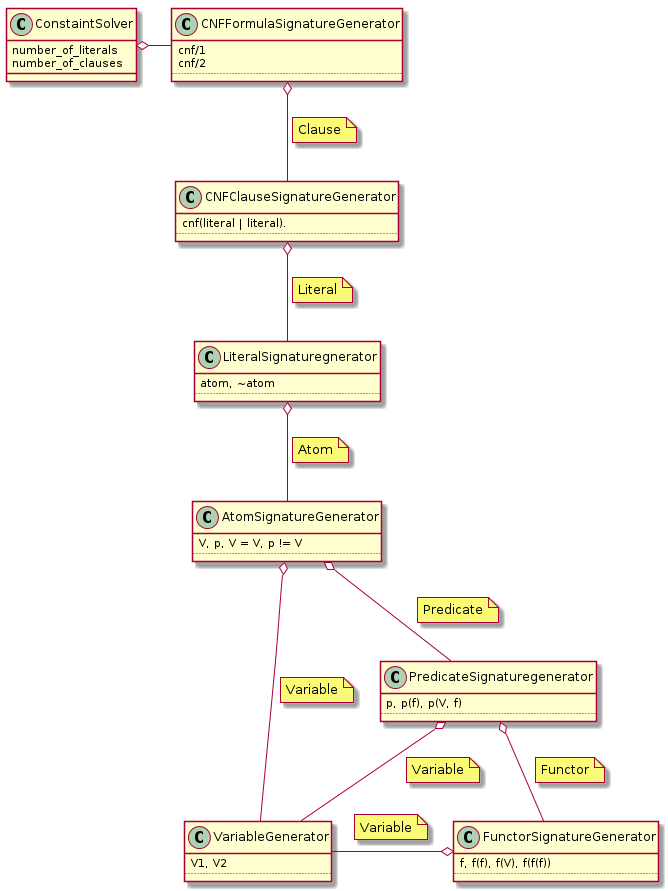
\includegraphics[width=0.7\textwidth]{logic-formula-generator/fol/cnf_signature_generators.png}
  \caption{Class diagram of generators in CNF formula generator}
  \label{pic:fol_signature_generator_class_diagram}
\end{centering}
\end{figure}

Manual creation of generators is required only in advanced case. To automate this process $CNFFormulaGnerator$ (picture \ref{pic:cnf_generator_class_diagram}) has been created. This is interface for user to create random CNF formulas that will automatically resolve user constraints and yield random formula. After creating formula from signature generators formula will be post processed - given random names and optionally negation sign. Generated formula can be then exported to file along with statistics about formula.

\begin{figure}[h]
\begin{centering}
  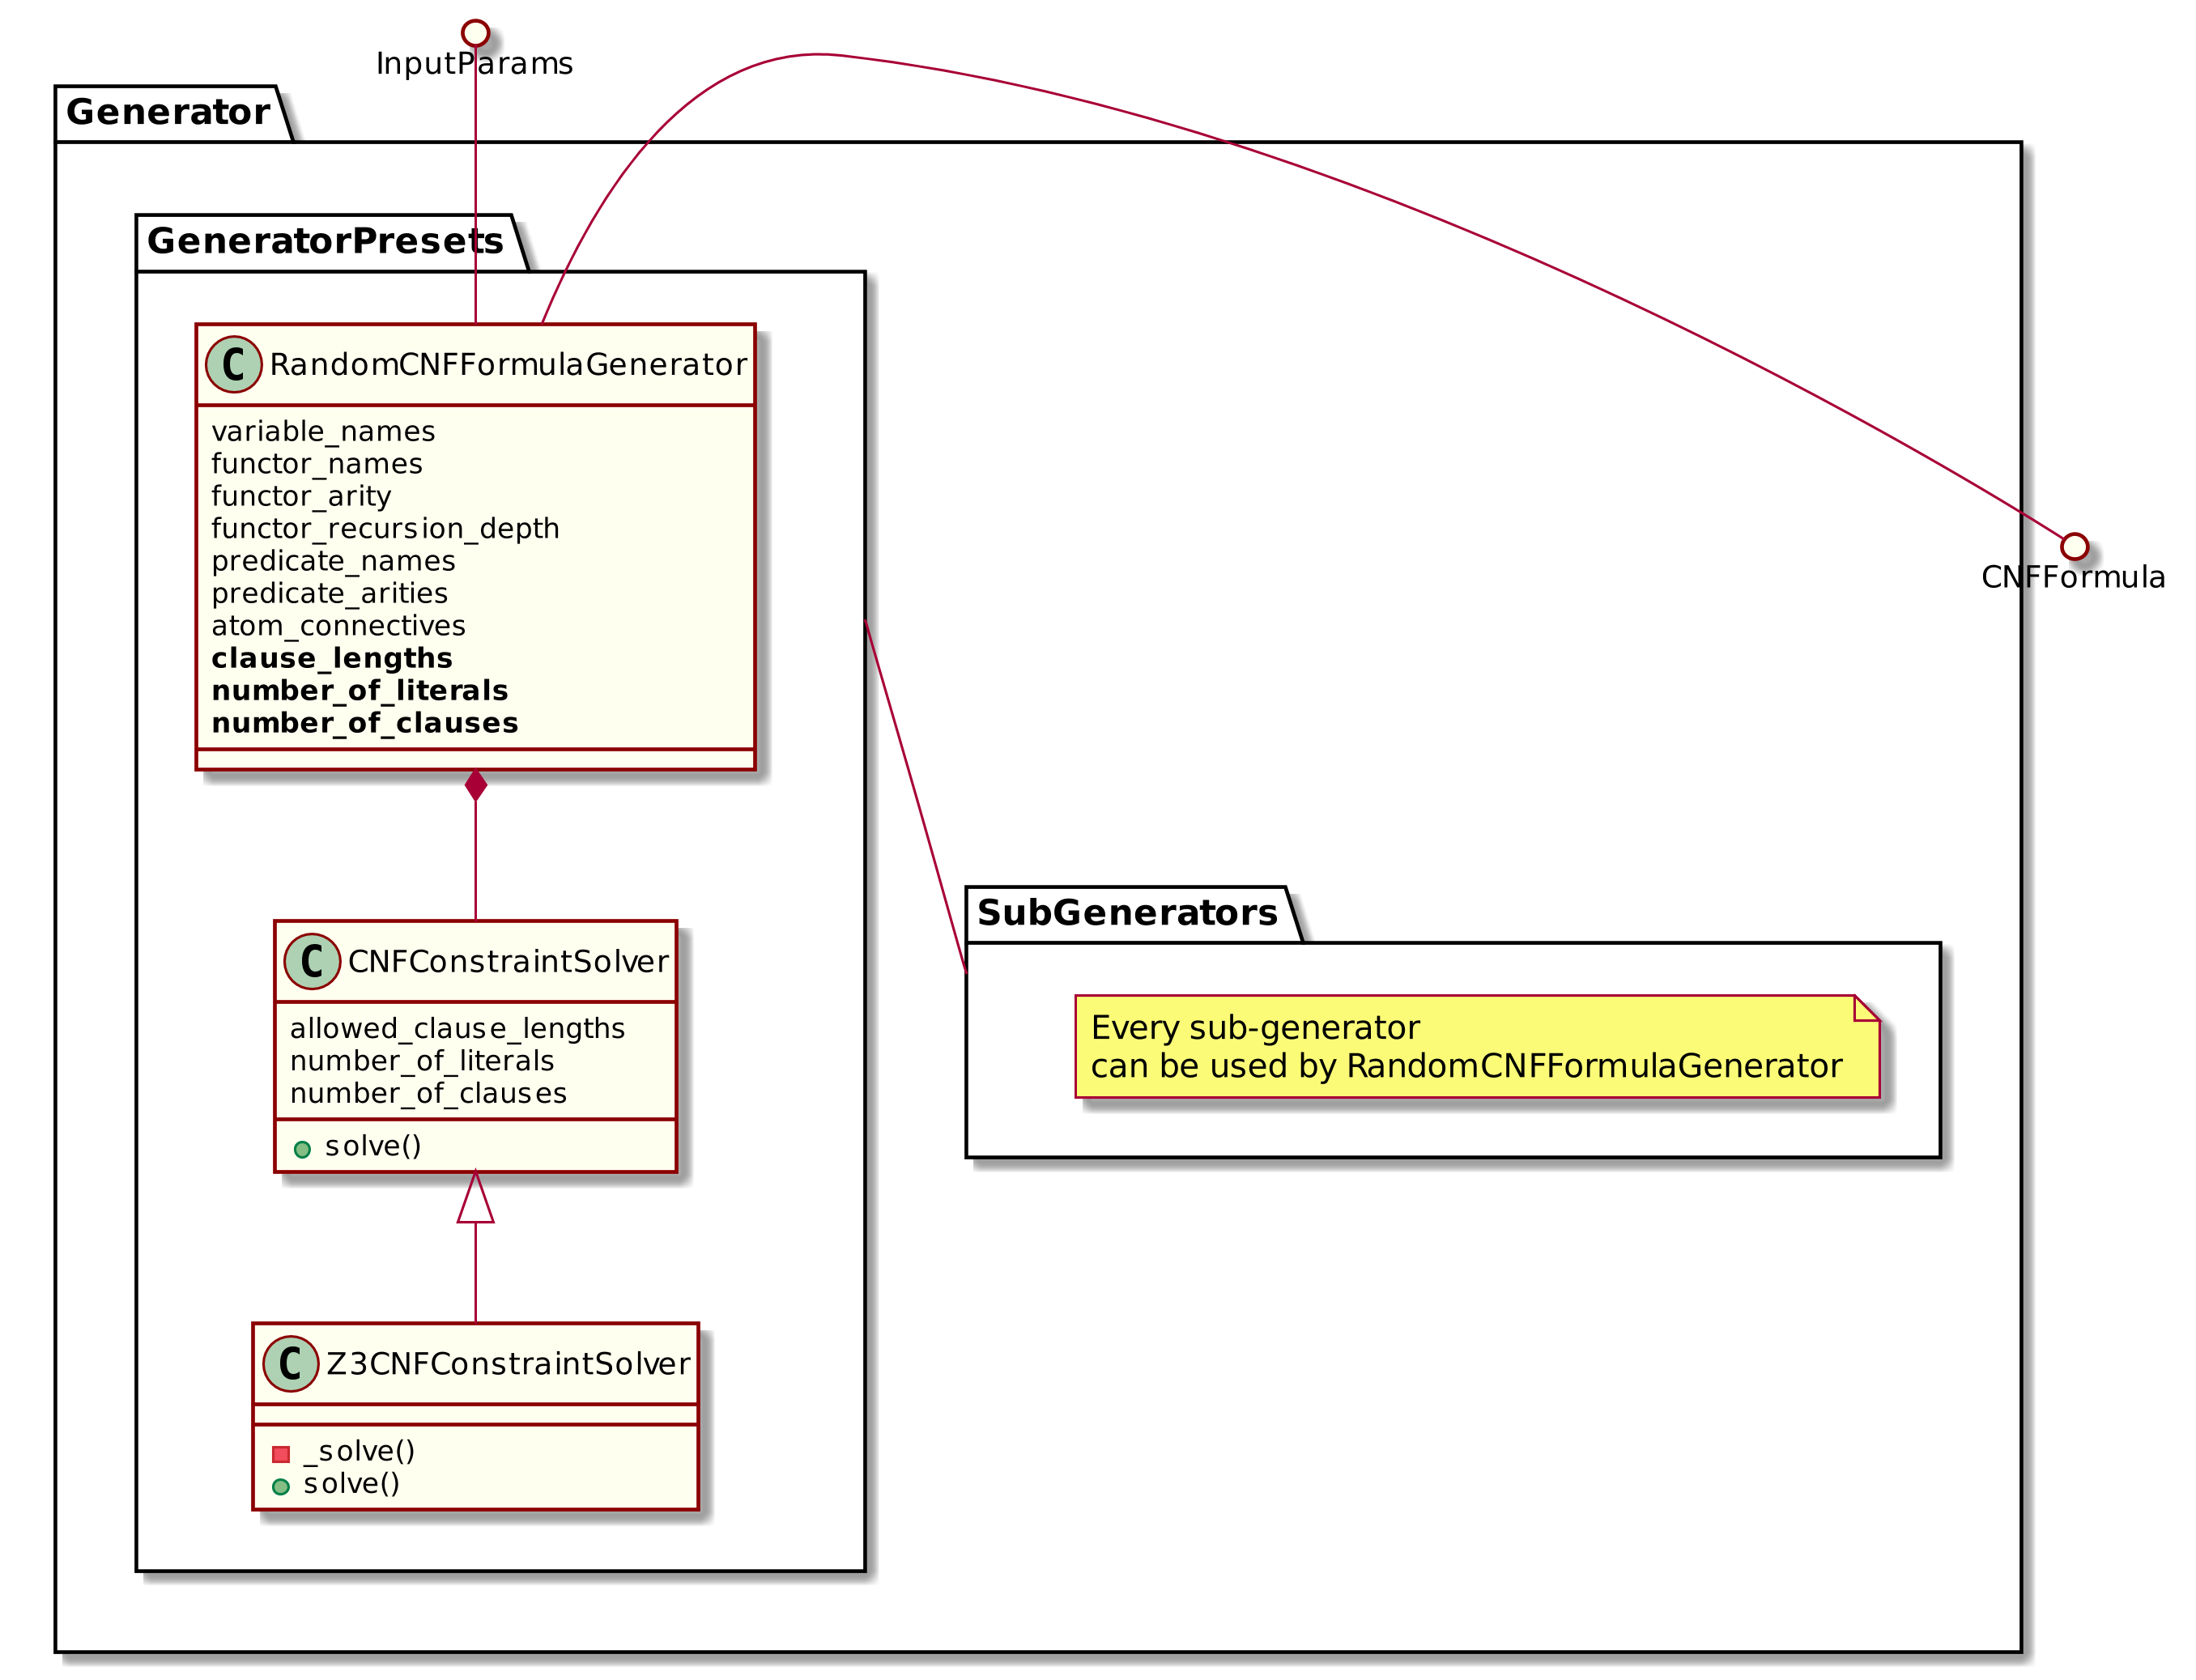
\includegraphics[width=\textwidth]{logic-formula-generator/cnf_formula_generator.png}
  \caption{Class diagram of CNF formula generator}
  \label{pic:cnf_generator_class_diagram}
\end{centering}
\end{figure}

% \subsection{Functor}
%
% Functor can contain variable or another functor.
% Given that
% $n$ is functor recursion depth,
% $a$ is functor arity,
% $f(n, a)$ number of functor signatures can be produced.
%
% \begin{align}
	% &f(n, a) =
	% \begin{cases}
    % a, \text{for } n = 0, \\
		% a \sum_{i=n}^{i=1} \sum_{j=a}^{j=0} f(n-i,a-j) \\
	% \end{cases}
% \end{align}
%
% Given that functor arity $a_f$ is in range $[a_{fmin}, a_{fmax}]$  and maximal recursion depth is $n_{max}$, $f(n_{max}, a_{fmin}, a_{fmax})$ number of functor signatures can be produced.
%
% \begin{align}
  % f(n_{max}, a_{fmin}, a_{fmax}) = \sum_{i=0}^{n_{max}} \sum_{j=a_{fmin}}^{a_{fmax}} f(i, j) \label{eq:functor}
% \end{align}
%
% \subsection{Predicates}
%
% Predicates can contain functors or variables.
% Given that $a_p$ is predicate arity, $P(a_p)$ number of predicate signatures can be produced.
%
% \begin{align}
	% P(a_p) &=
	% \begin{cases}
		% 1, \text{for } a_p = 0 \\
		% (f(n_{max}, a_{fmin}, a_{fmax}) + 1)^{a_p}, \\
	% \end{cases}
% \end{align}
%
% Given that predicate arity $a_p$ is in range $[a_{pmin}, a_{pmax}]$, $p(a_{fmin}, a_{fmax})$ number of functor signatures can be produced.
%
% \begin{align}
  % p(a_{pmin}, a_{pmax}) = \sum_{i=a_{pmin}}^{a_{pmax}} p(i) \label{eq:predicate}
% \end{align}
%
% \subsection{Atoms}
%
% Atom can contain only predicate. Single variable on its own is not an atom. Atom connects items with binary mathematical connective: $=$ or $!=$ or $\emptyset$ (no connective).
% Given that atom $connective$, $A(connective)$ atom signatures can be produced.
%
% \begin{align}
	% A(connective) &=
  % \begin{cases}
    % p(a_{pmin}, a_{pmax})^{2}, \text{for } connective \in \{'=', '!='\} \\
    % p(a_{pmin}, a_{pmax}), \text{for } connective \in \{\emptyset\} \label{eq:atom}
  % \end{cases}
% \end{align}
%
% \subsection{Literals}
%
% Literal is atom or its negation.
%
% \begin{align}
  % L = A(AllowedConnectives) * 2 \label{eq:literal}
% \end{align}
%
% \subsection{CNF Clause}
%
% Clause $C$ can contain only atoms $A$. The order of atoms is irrelevant $C = \{a1, a2, \dots\}$
%
% Given that
% clause length $l$ and
% set of unique atoms $A = \{a1, a2, \dots\}$, $\forall_{i,j \in L} i \neq j$
% $C(a)$ clauses can be produced. Atoms can repeat.
%
% \begin{align}
  % C(l) = \binom{A + l - 1}{l}
% \end{align}
%
% Given that clause length $l$ is in range $[l_{min}, l_{max}]$
%
% \begin{align}
  % C(l_{min}, l_{max}) = \sum_{i=l_{min}}^{i=l_{max}} C(i) \label{eq:clause}
% \end{align}
%
% \subsection{CNF formulas}
%
% Given that
% formula contains $x$ clauses and
% set of unique clauses $C = \{c1,c2, \dots\}$
% $F$ formulas can be produced. Clauses can repeat.
%
% \begin{align}
  % &F_{cnf}(x) = C(l)^{x} \label{eq:cnfformula}
% \end{align}
